\documentclass{ctexart}
    \usepackage{mathrsfs}
    \usepackage{multirow}
    \usepackage{graphicx}
    \usepackage{array}
    \usepackage{makecell}
    \usepackage{amsmath}
    \usepackage{booktabs}
    \usepackage{float}
    \newcommand\mgape[1]{\gape{$\vcenter{\hbox{#1}}$}}

    \author{钱思天\ 1600011388 No.8}
    \title{实验二十二:迈克尔逊干涉仪\ 实验报告}
    \begin{document}
      \maketitle
      \section{第一部分实验内容}
      \subsection{调节迈克尔逊干涉仪}
      \paragraph{1}首先,打开激光器,大致调节使之与$G_1$镜成$45^\circ$
      \paragraph{2}取小孔于光路上,调节激光器俯仰及小孔高低,使激光通过小孔射向迈克尔逊干涉仪。在此调解过程中,“远调(激光器)俯仰,近调(小孔)高低”。
      \paragraph{3}待小孔置于激光器光路中后,观察小孔屏上经$M_1$与$M_2$反射所成像的位置,调节两平面镜后的三个调节螺丝,使得所成的像中的最亮点与小孔重合,达到准直。
      \subsection{圆条纹与椭圆条纹的调节}
      \paragraph{1}首先,在小孔与干涉仪间加一短焦距小透镜$L$,使光束汇聚为一点光源且均匀照亮$M_2$,在观察屏$E$上便可初步观察到干涉条纹。
      \paragraph{2}调节粗调螺旋至出现直线条纹,而后,调节两个$M_2$调节旋钮$U_2$,使得视野里仅出现亮区,便使$M_1$与$M_2$基本重合。
      \paragraph{3}此后,调节粗调旋钮,便可在观察屏上观察到一系列同心的圆形条纹。
      \paragraph{4}此时,若将观察屏水平旋转一小角度使其与光路不垂直,便可观察到椭圆条纹。
      \paragraph{变化规律}从视野全亮计,(Ⅰ)若将$M_1$调远,则圆环外吐,调远后再调近,则圆环内吞;(Ⅱ)若将$M_1$调近,则圆环外吐,调近后再调远,则圆环内吞。
      \paragraph{解释}(Ⅰ)视野全亮,代表着$M_1$与$M_2$的像基本重合,且连线与观察屏垂直。(Ⅱ)此时,若将$M_1$调远,则两光束光程差增加,从而使得干涉条纹数目增多,圆环外吐,再将$M_1$调近,光程差减小,圆环内吞。(Ⅲ)若将$M_1$调近,则光程差也增加,圆环外吐,再将$M_1$调远,光程差减小,圆环内吞。
      \subsection{直条纹与双曲线条纹的调节}
      \paragraph{1}承接上一实验,调节粗调螺旋至视野全亮,而后,调节调节两个$M_2$调节旋钮$U_2$,便使得视野出现间距适当的直条纹。
      \paragraph{2}此时若将观察屏水平旋转一小角度使其与光路不垂直,便可观察到双曲线条纹。
      \subsection{严格等倾}
      \paragraph{1}承接实验2,将一毛玻璃置于光路中,使点光源变为一拓展光源,旋下观察屏,用肉眼作为观察仪器。
      \paragraph{2}与实验2类似地,调节使得两镜之像基本重合,而后调节粗调螺旋,观察所成干涉圆环。
      \paragraph{3}上下左右平行地移动观察,使得在不同位置观察下,干涉条纹仅仅有位置上的改变,而不改变其图案(即无圆环的吞吐),便完成了严格等倾的调节。
      \paragraph{解释}(Ⅰ)等倾干涉意味着,等光程位置为等倾角入射,根据几何知识,可知其干涉花样为一簇同心圆,且随着$M_1$的调近调远花样会有圆环的吞吐。(Ⅱ)但是,改用扩展光源的等倾条纹,实为定域干涉,域为无穷远点,因此,完成严格等倾后,平行地改动观察位置,也不会改变总图样的形状(中心条纹级次不变),只是改变干涉花样的位置。
      \paragraph{等厚}
      \paragraph{1}仍采用肉眼作为观察器材,在实验4的基础上,与实验3类似地,调节到出现合适间隔的直线条纹。
      \paragraph{2}此时,改变$M_1$镜的位置,会发现干涉花样由直变曲的现象。
      \paragraph{解释}(Ⅰ)与实验3类似的,从视野最亮处,调节旋钮$U_2$,则两镜之像间会出现夹角,从而达成等厚干涉出现的条件,出现直条纹。(Ⅱ)此时若前后移动$M_1$,则之中会出现光程差,与未调节两镜平行时情况类似。故而干涉条纹会出现由弯变直。
      \subsection{白光等厚干涉}
      \paragraph{1}在实验5的基础上,光路中引入白光作为光源。
      \paragraph{2}在实验5的直条纹附近,调节粗调螺旋,寻找到出现白光干涉花样的位置。
      \paragraph{3}在白光干涉花样位置附近,进一步使用细调螺旋,调节到白光干涉花样的位置。
      \paragraph{现象}白光干涉花样中心主极大为白色亮纹,两旁黑色暗纹。在干涉区域的外端还可看到彩虹状的不同色光的主极大。以中心白色主极大条纹计,内红外紫。
      \paragraph{读数}出现白光干涉的位置:$$ d=33.05921mm$$
      \section{第二部分实验内容}
      \subsection{测量空气折射率}
      \subsubsection{实验数据}
      % Table generated by Excel2LaTeX from sheet 'Sheet1'
\begin{table}[htbp]
  \centering
  \caption{所用常数}
  \resizebox{\textwidth}{!}
  {
    \begin{tabular}{llllr}
    物理量   & 小气室厚度D & He-Ne激光波长$\lambda$ & 大气压数值$p_0$ & \multicolumn{1}{l}{间隔环数N} \\
    值     & 4.00cm & 632.8nm & 101.2kpa & 2 \\
    \end{tabular}%
  }
  \label{tab:addlabel}%
\end{table}%
% Table generated by Excel2LaTeX from sheet 'Sheet1'
\begin{table}[htbp]
  \centering
  \caption{间隔两个环气压值}
  \resizebox{\textwidth}{!}
  {
    \begin{tabular}{lrrrrrrrrr}
    各次测量气压值 & \multicolumn{1}{l}{$p_0$} & \multicolumn{1}{l}{$p_1$} & \multicolumn{1}{l}{$p_2$} & \multicolumn{1}{l}{$p_3$} & \multicolumn{1}{l}{$p_4$} & \multicolumn{1}{l}{$p_5$} & \multicolumn{1}{l}{$p_6$} & \multicolumn{1}{l}{$p_7$} & \multicolumn{1}{l}{$p_8$} \\
    单位:hpa & 1012  & 1071  & 1134  & 1194  & 1260  & 1319  & 1378  & 1439  & 1500 \\
    \end{tabular}%
  }
  \label{tab:addlabel}%
\end{table}%
    \subsection{计算}
    运用公式:
    $$n=1+\frac{N\lambda}{2D}\cdot\frac{p}{|\Delta p|}$$
    可知,次数$i$与气压读数$p_i$应成线性关系,$\Delta p$为其斜率。
    将实测数据作图,有:
    \begin{figure}[H]
      \centering
      \caption{各次气压读数数据图}
      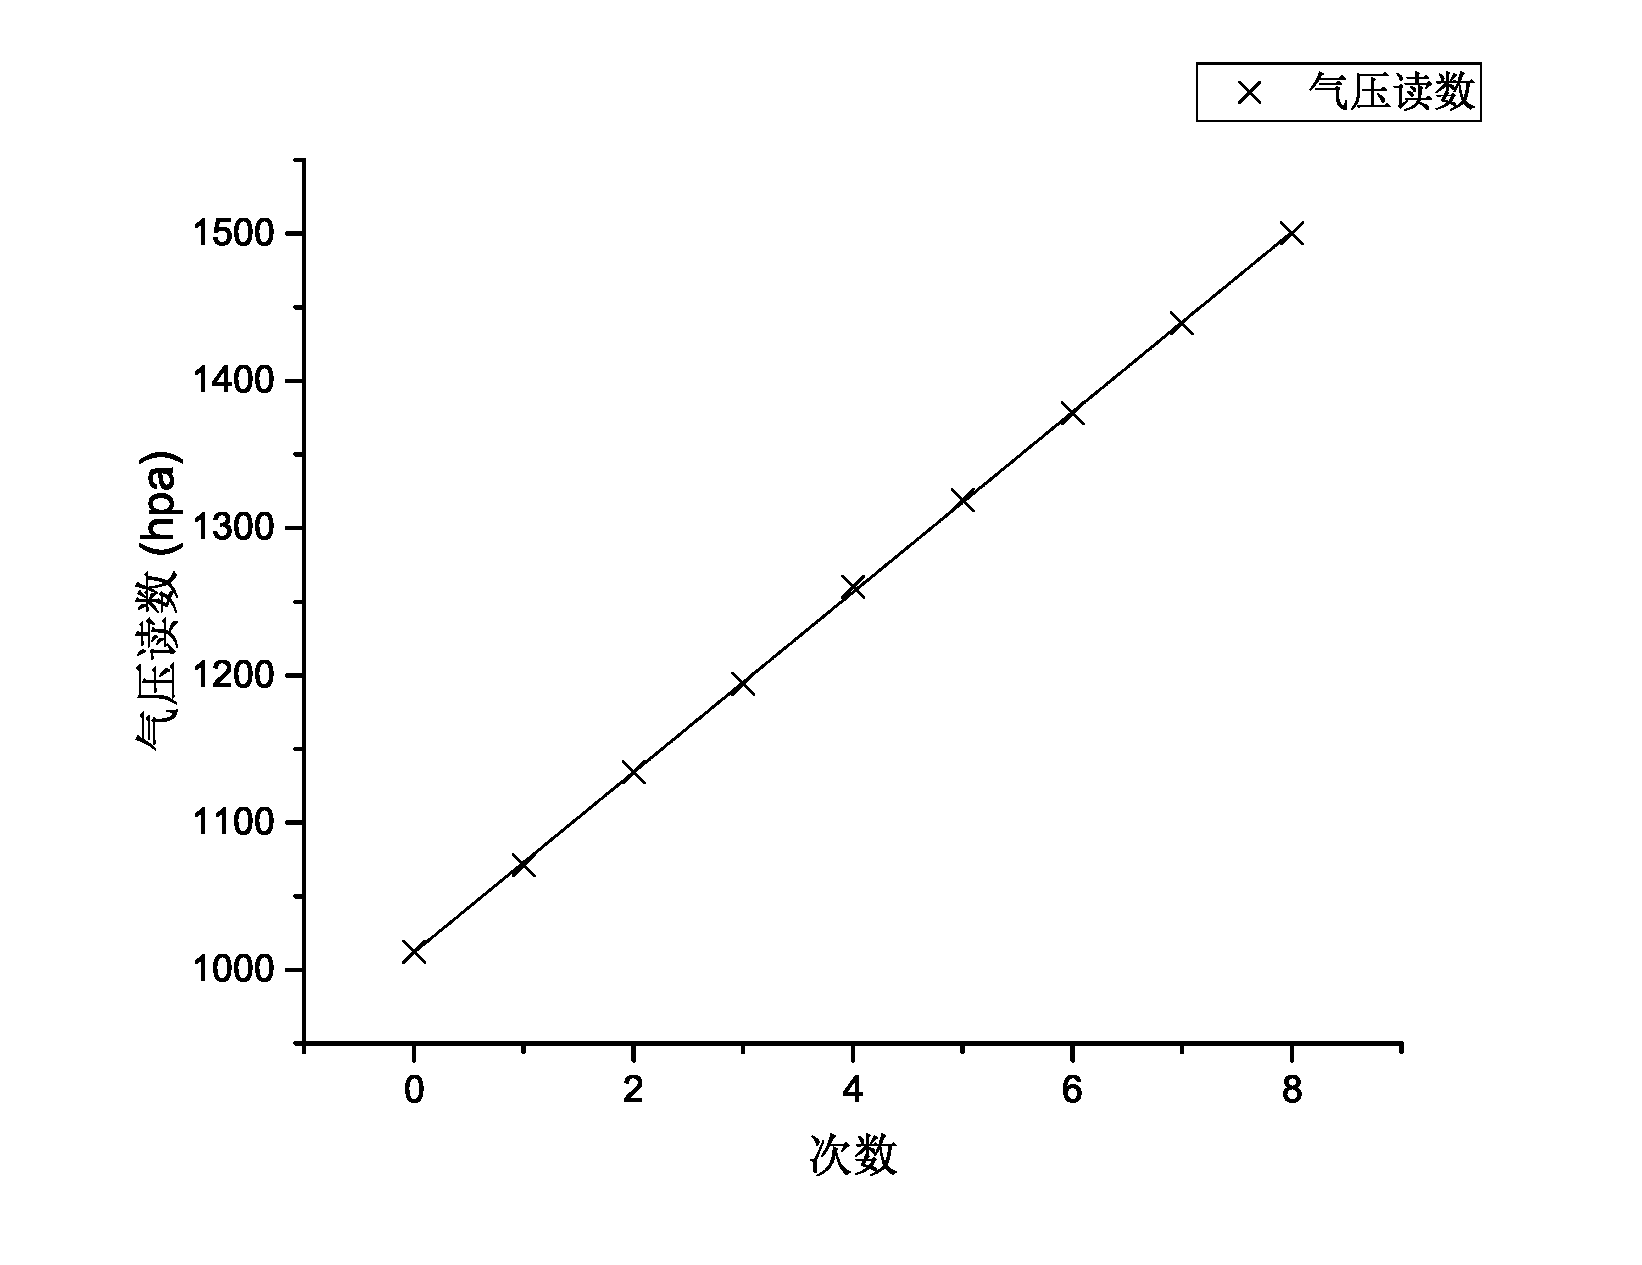
\includegraphics[width=\textwidth]{1}
      \label{fig:digit}
    \end{figure}
    计算有$r\approx0.9999$,故为线性关系。
    设回归方程满足$$p_i=\Delta p\cdot i+p_0$$
    则有公式$$\Delta p=\frac{\sum\limits_{i=0}^{8}{({p}_i-\bar{p})(i-\bar{i})}}{\sum\limits_{i=0}^{8}{(i-\bar{i})^2}}=61.15(hpa)$$
      $$\sigma_{\Delta p}=\frac{\sigma_{p}}{\sqrt{\sum\limits_{i=0}^{8}{(i-\bar i)^2}}}=\Delta p \cdot \sqrt{\frac{1-r^2}{9-2}}=0.23(hpa)$$
      代入原公式,有
      $$n=1.0002618$$
      $$\sigma_n=0.0000009$$
      故:$$n\pm\sigma_n=1.0002618\pm0.0000009$$

      \subsection{测量压电陶瓷的压电常量}
      \subsubsection{实验数据}
      % Table generated by Excel2LaTeX from sheet 'Sheet1'
\begin{table}[htbp]
  \centering
  \caption{常数数据}
  
    \begin{tabular}{llll}
    物理量   & 长度L   & 壁厚t   & He-Ne激光波长 \\
    值     & 46mm  & 1.0mm & 632.8nm \\
    \end{tabular}%

  \label{tab:addlabel}%
\end{table}%
    % Table generated by Excel2LaTeX from sheet 'Sheet1'
\begin{table}[htbp]
  \centering
  \caption{各次电压测量值}
  
    \begin{tabular}{lrrrrrr}
    各次测量电压值 & \multicolumn{1}{l}{U1} & \multicolumn{1}{l}{U2} & \multicolumn{1}{l}{U3} & \multicolumn{1}{l}{U4} & \multicolumn{1}{l}{U5} & \multicolumn{1}{l}{U6} \\
    单位V   & -66.9 & -42.0   & -15.9 & 8.2   & 32.6  & 55.1 \\
    \end{tabular}%
  
  \label{tab:addlabel}%
\end{table}%
    \subsubsection{计算}
    运用公式:
    $$\Delta L=d_{21} (\frac{L}t)U_f$$
    可知,长度改变量$\Delta L$与电压读数$U_f$应成线性关系,且有$\Delta L_i=\frac{\lambda}2\times i$,故次数$i$与读数${U_f}_i$成线性关系,$\frac{1}{d_{21} (\frac{L}t)}\cdot \frac{\lambda}2$为其斜率。
    将实测数据作图,有:
    \begin{figure}[H]
      \centering
      \caption{各次电压读数数据图}
      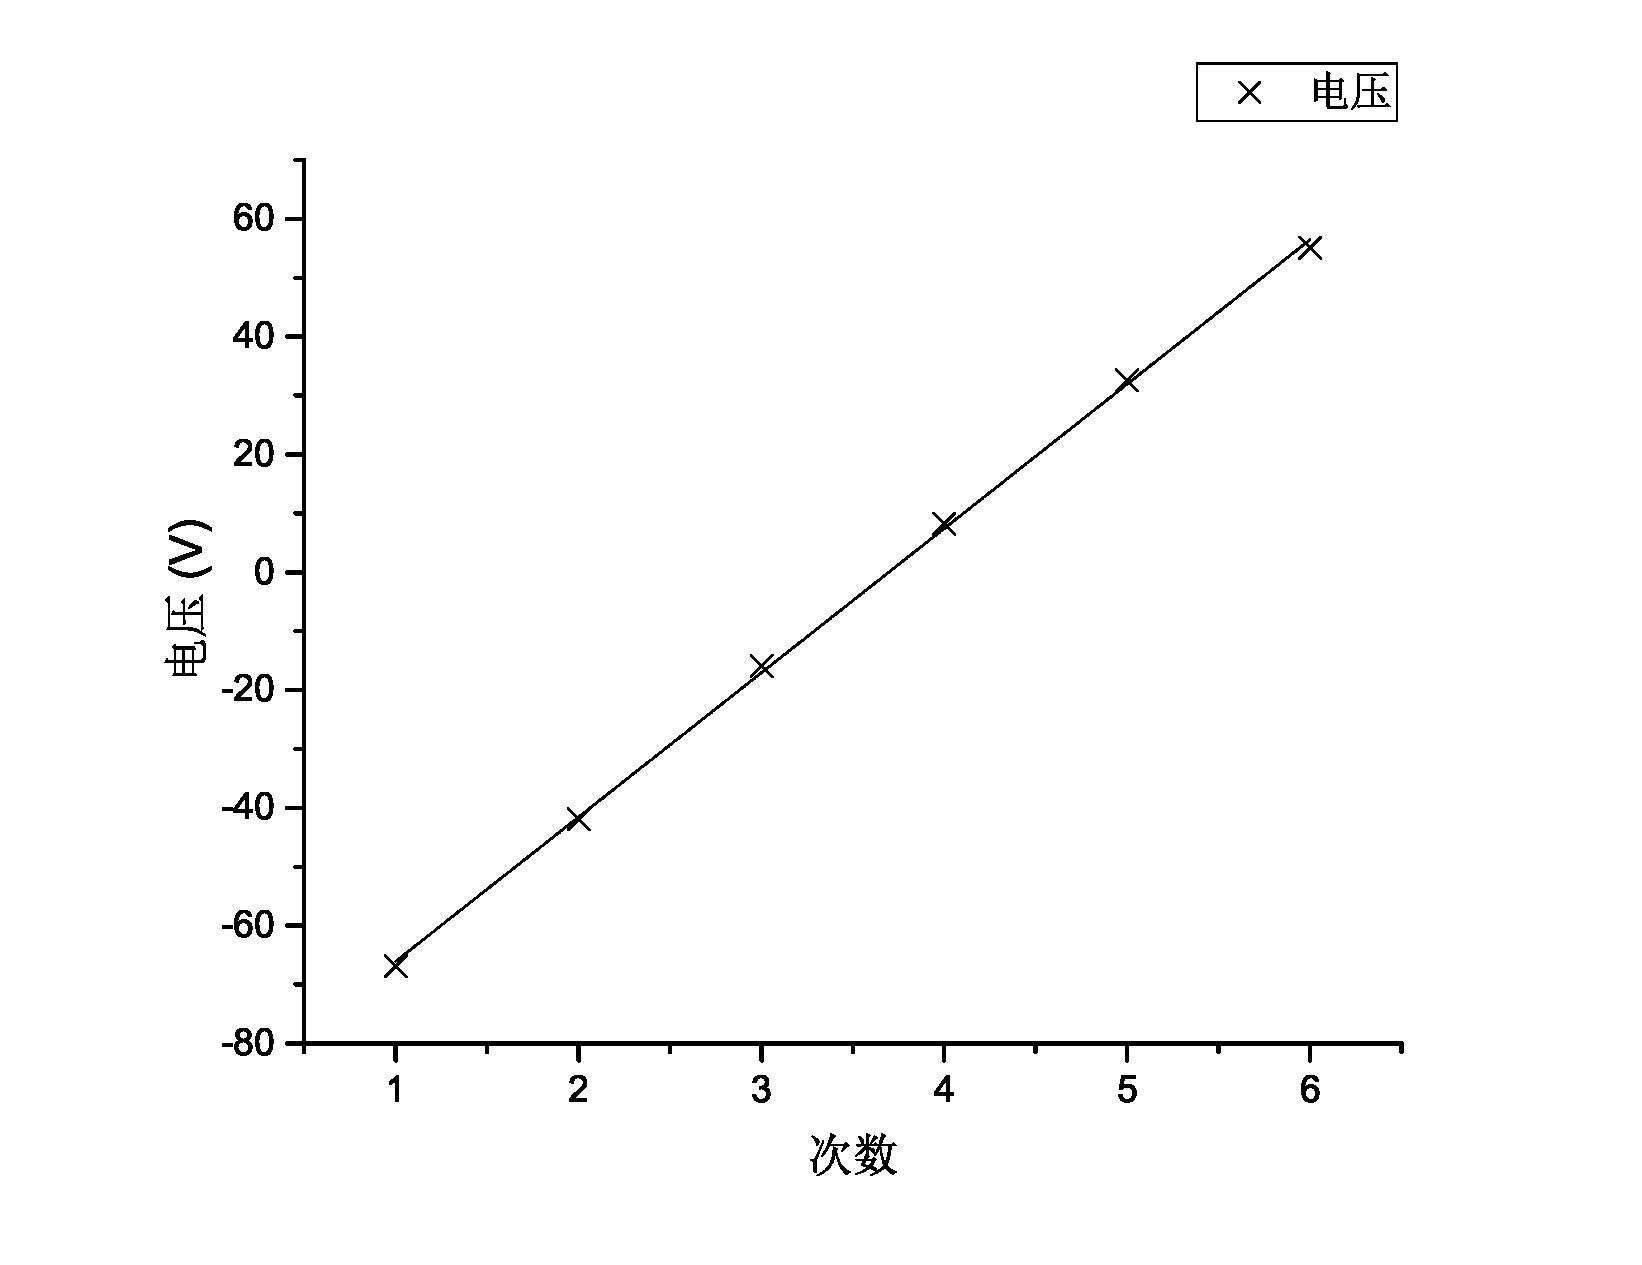
\includegraphics[width=\textwidth]{2}
      \label{fig:digit}
    \end{figure}
    计算有$r\approx0.9998$,故为线性关系。
    设回归方程满足$$U_i=k\cdot i+U_0$$
    则有公式$$k=\frac{\sum\limits_{i=1}^{6}{({U}_i-\bar{U})(i-\bar{i})}}{\sum\limits_{i=1}^{6}{(i-\bar{i})^2}}=24.52(V)$$
      $$\sigma_{k}=\frac{\sigma_{U}}{\sqrt{\sum\limits_{i=0}^{8}{(i-\bar i)^2}}}=k \cdot \sqrt{\frac{1-r^2}{6-2}}=0.26(V)$$
      代入原公式,有
      
      $$d_{21}=2.81\times10^{-10}(m/V)$$
      $$\sigma_{d_{21}}=0.03\times10^{-10}(m/V)$$

      故:$$d_{21}\pm\sigma_{d_{21}}=2.81\pm0.03(10^{-10}m/V)$$
      \section{收获与感想}
      这次实验的时间安排对我来说非常的巧妙,因为我将将在光学课上学过了迈克尔逊干涉仪。

      光学课上,老师对迈克尔逊干涉仪可以说是赞不绝口。而当我预习实验时,也不由得为它的精妙所感叹。这台并不能算大的仪器,竟然拥有着10nm的精度。从寻找以太,到LIGO,都有着迈克尔逊干涉仪的身影。

      实际操作起来,我发现调节迈克尔逊干涉仪的过程也是非常有趣的,种种干涉花样接踵而至,亲眼见证等厚,等倾干涉条纹,看到彩虹般的白光干涉。

      当然,实验中,我也收获了很多。比如在调节迈克尔逊干涉仪的过程中,各螺丝要前后各留出一定的位置以方便进一步的调节,这些都是我需要注意的。以及我深刻感受到了,哪怕是轻微的脚步声,也会对实验的效果产生很大的影响,这启发了我要端正z

      在今后的实验课中,我也会努力提高自己的实验能力,端正自己的实验态度。
    \end{document}